\chapter{Выполнение работы}

\section{Расчётные соотношения}

В списке ниже в скобках указаны идентификаторы соответствующих величин, рассчитываемые в программе.

\begin{itemize}[$\bullet$]
	\item Объем выборки $n$ ~~~(\texttt{N})

	\item точечная оценка математического ожидания $\hat{\mu}(\overrightarrow{x_n})$ ~~~(\texttt{mu\_hat})
	
	\begin{equation}
		\hat{\mu}(\overrightarrow{x_n}) = \frac{1}{n} \sum_{i=1}^{n} x_i
	\end{equation}

	\item точечная оценка дисперсии $S^2(\overrightarrow{x_n})$ ~~~(\texttt{S\_2})
	
	\begin{equation}
		S^2(\overrightarrow{x_n}) = \frac{1}{n-1} \sum_{i=1}^{n} [x_i - \hat{\mu}(\overrightarrow{x_n})]^2
	\end{equation}

	\item границы $\gamma$-доверительного интервала для математического ожидания 
	
	(\texttt{mu\_hat\_low}, \texttt{mu\_hat\_high})
	
	\begin{equation}
		\underline{\mu}(\overrightarrow{x_n}) = \hat{\mu}(\overrightarrow{x_n}) + \sqrt{\frac{S^2(\overrightarrow{x_n})}{n}} \cdot t_{\frac{1 - \gamma}{2}}(n-1)
	\end{equation}

	\begin{equation}
		\overline{\mu}(\overrightarrow{x_n}) = \hat{\mu}(\overrightarrow{x_n}) + \sqrt{\frac{S^2(\overrightarrow{x_n})}{n}} \cdot t_{\frac{1 + \gamma}{2}}(n-1),
	\end{equation}

	где $t_{\alpha}(m)$ -- $\alpha$-квантиль распределения Стьюдента с $m$ степенями свободы.

	\item границы $\gamma$-доверительного интервала для дисперсии ~(\texttt{S\_2\_low}, \texttt{S\_2\_high})
	
	\begin{equation}
		\underline{\sigma}^2(\overrightarrow{x_n}) = S^2(\overrightarrow{x_n}) \cdot \sqrt{\frac{n-1}{\chi^2_{\frac{1 + \gamma}{2}}(n-1)}}
	\end{equation}

	\begin{equation}
		\overline{\sigma}^2(\overrightarrow{x_n}) = S^2(\overrightarrow{x_n}) \cdot \sqrt{\frac{n-1}{\chi^2_{\frac{1 - \gamma}{2}}(n-1)}},
	\end{equation}

	где $\chi^2_{\alpha}(m)$ -- верхняя $\alpha$-квантиль распределения хи-квадрат с $m$ степенями свободы.

\end{itemize}

\clearpage

\section{Определение $\gamma$-доверительного интервала}

\textbf{Пусть}:

\begin{enumerate}[a)]
	\item $X$ -- случайная величина, закон распределения которой зависит от неизвестного параметра $\theta$,
	\item $\overrightarrow{X}$ -- случайная выборка из $X$.
\end{enumerate}

\textbf{Определение}: \underline{интервальной оценкой уровня $\gamma$ параметра $\theta$} называется интервал со случайными границами, который накрывает теоретическое значение параметра $\theta$ с вероятностью $\gamma$.

\textbf{Определение}: \underline{$\gamma$-доверительным интервалом} (доверительным интервалом уровня $\gamma$) параметра $\theta$ называют реализацию (выборочное значение) интервальной оценки уровня $\gamma$ для этого параметра, то есть интервал с детерминированными границами $(\underline{\theta}(\overrightarrow{x}), \overline{\theta}(\overrightarrow{x}))$.

\clearpage

\section{Результаты работы}

\begin{table}
	\centering
	\begin{tabular}{|c|c|}
		\hline
		\textbf{~~Величина~~} & \textbf{~~Значение~~} \\
		\hline
		$n$ & \texttt{120} \\
		$\hat{\mu}$ & \texttt{0.23} \\
		$S^2$ & \texttt{1.04} \\
		$(\underline{\mu}, \overline{\mu})$ & (\texttt{0.07}, \texttt{0.39}) \\
		$(\underline{\sigma}^2, \overline{\sigma}^2)$ & (\texttt{0.94}, \texttt{1.17}) \\
		\hline
	\end{tabular}
	\caption{Результаты расчетов параметров выборки}
\end{table}

\begin{figure}
	\centering	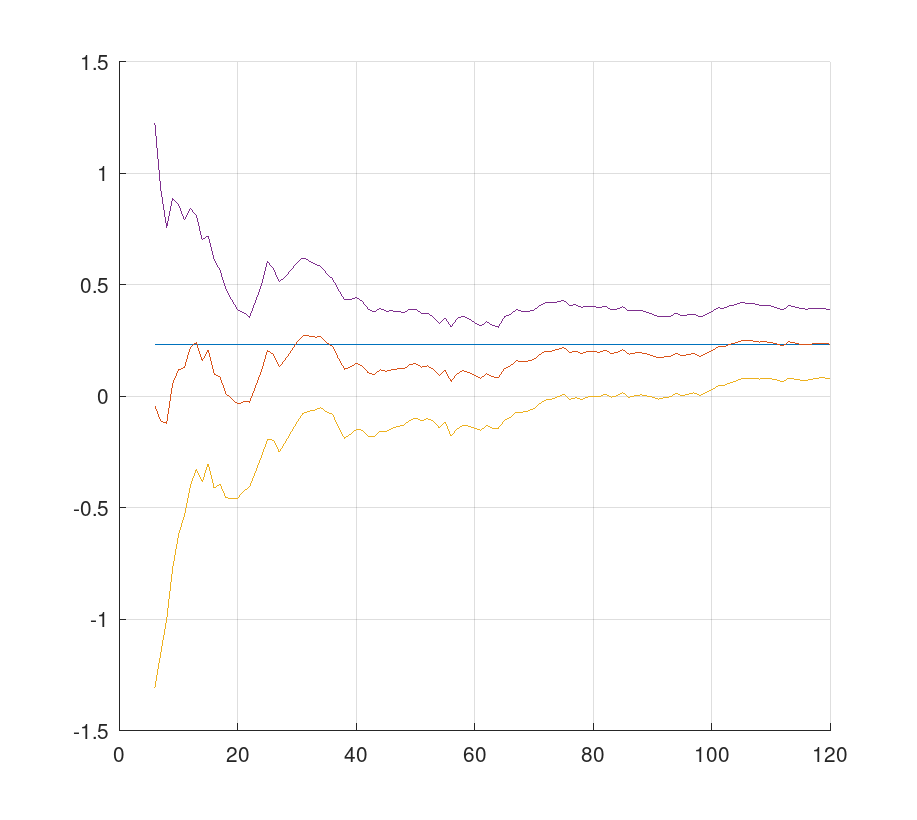
\includegraphics[width=0.8\linewidth]{img/screenshot001}
	\caption{Графики зависимостей нижней и верхней границ интервала для математического ожидания от объема выборки при $n = 6\dots120$}
	\label{fig:screenshot001}
\end{figure}

\begin{figure}
	\centering
	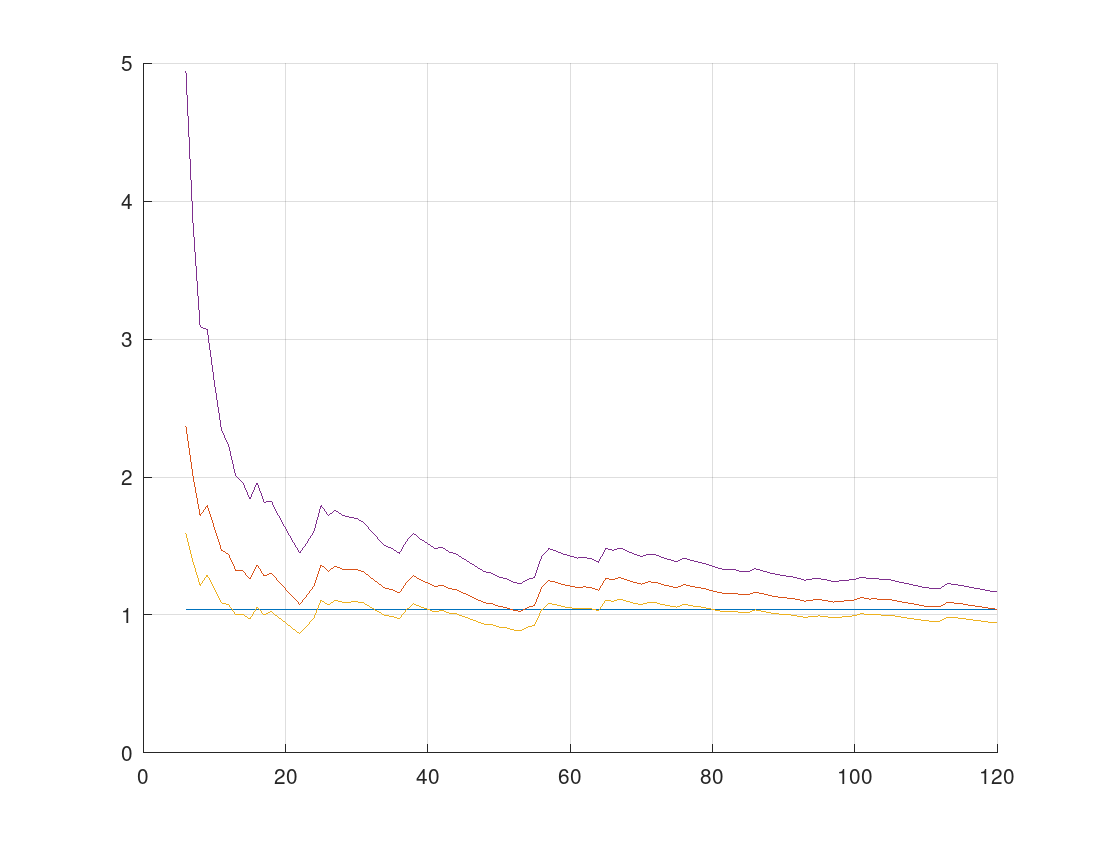
\includegraphics[width=\linewidth]{img/screenshot002}
	\caption{Графики зависимостей нижней и верхней границ интервала для дисперсии от объема выборки при $n = 6\dots120$}
	\label{fig:screenshot002}
\end{figure}

\clearpage

\section{Текст программы}

\begin{lstlisting}
#!/bin/octave -qf

pkg load statistics

X = [-0.45, -0.33, 2.92, -1.25, -1.20, 0.05, -0.53, -0.19, 1.49, 0.67, 0.22, 1.23, 0.50, -0.92, 0.90, -1.52, -0.15, -1.24, -0.47, -0.45, 0.18, -0.05, 1.58, 1.74, 2.37, -0.24, -1.34, 1.05, 1.28, 1.37, 1.18, 0.22, 0.11, 0.28, -0.64, -0.39, -1.77, -1.61, 0.47, 0.77, -0.27, -1.19, -0.25, 1.04, -0.16, 0.42, 0.29, 0.10, 1.04, 0.43, -0.67, 0.41, -0.62, -1.49, 1.46, -2.77, 2.09, 0.88, -0.36, -0.71, -0.62, 1.34, -0.78, -0.15, 2.69, 0.92, 1.68, -0.12, 0.34, 0.74, 1.72, 1.24, 0.23, 0.76, 0.87, -1.52, 0.63, -0.56, 0.83, 0.31, -0.18, 0.99, -1.01, 0.58, 1.21, -1.51, 0.65, 0.35, -0.37, -0.50, -0.73, 0.63, 0.33, 1.56, -0.98, 0.85, 0.56, -1.07, 1.47, 1.44, 1.91, 0.24, 1.34, 0.99, 1.27, 0.11, 0.22, -0.25, 0.35, -0.03, -0.56, -0.79, 2.41, -0.45, -0.44, 0.07, 0.64, 0.69, 0.10, -0.28];

gam = 0.9;
n = length(X)

function mu = mu_hat(X)
    mu = sum(X) / length(X);
endfunction

function s2 = S_2(X)
    s2 = sum((X - mu_hat(X)) .^ 2)/(length(X) - 1);
endfunction

function mu = mu_hat_low(X, gam)
    n = length(X);
    mu = mu_hat(X) + sqrt(S_2(X) / n) * tinv([(1 - gam)/2], n - 1);
endfunction

function mu = mu_hat_high(X, gam)
    n = length(X);
    mu = mu_hat(X) + sqrt(S_2(X) / n) * tinv([(1 + gam)/2], n - 1);
endfunction

function s2 = S_2_low(X, gam)
    n = length(X);
    s2 = S_2(X) * sqrt((n - 1)/chi2inv([(1 + gam)/2], n - 1));
endfunction

function s2 = S_2_high(X, gam)
    n = length(X);
    s2 = S_2(X) * sqrt((n - 1)/chi2inv([(1 - gam)/2], n - 1));
endfunction
\end{lstlisting}

\clearpage

\begin{lstlisting}[firstnumber=37]
mu_hat(X)
S_2(X)
mu_hat_low(X, gam)
mu_hat_high(X, gam)
S_2_low(X, gam)
S_2_high(X, gam)

N = zeros(1, n);
y_mu_hat = zeros(1, n);
y_mu_hat_n = zeros(1, n);
y_mu_hat_low = zeros(1, n);
y_mu_hat_high = zeros(1, n);
z_S_2 = zeros(1, n);
z_S_2_n = zeros(1, n);
z_S_2_low = zeros(1, n);
z_S_2_high = zeros(1, n);
for i = 1:n
    Xn = X(1:i);
    N(1, i) = i;
	y_mu_hat(1, i) = mu_hat(X);
	y_mu_hat_n(1, i) = mu_hat(Xn);
	y_mu_hat_low(1, i) = mu_hat_low(Xn, gam);
	y_mu_hat_high(1, i) = mu_hat_high(Xn, gam);
	z_S_2(1, i) = S_2(X);
	z_S_2_n(1, i) = S_2(Xn);
	z_S_2_low(1, i) = S_2_low(Xn, gam);
	z_S_2_high(1, i) = S_2_high(Xn, gam);
endfor;

skip_n = 6;
hold on
plot(N(1, skip_n:n), y_mu_hat(1, skip_n:n))
plot(N(1, skip_n:n), y_mu_hat_n(1, skip_n:n))
plot(N(1, skip_n:n), y_mu_hat_low(1, skip_n:n))
plot(N(1, skip_n:n), y_mu_hat_high(1, skip_n:n))
hold off
pause;

hold on
plot(N(1, skip_n:n), z_S_2(1, skip_n:n))
plot(N(1, skip_n:n), z_S_2_n(1, skip_n:n))
plot(N(1, skip_n:n), z_S_2_low(1, skip_n:n))
plot(N(1, skip_n:n), z_S_2_high(1, skip_n:n))
hold off
pause;
\end{lstlisting}

%\section{Выборка для заданий 1-2}

%X = (-0.45, -0.33, 2.92, -1.25, -1.20, 0.05, -0.53, -0.19, 1.49, 0.67, 0.22, 1.23, 0.50, -0.92, 0.90, -1.52, -0.15, -1.24, -0.47, -0.45, 0.18, -0.05, 1.58, 1.74, 2.37, -0.24, -1.34, 1.05, 1.28, 1.37, 1.18, 0.22, 0.11, 0.28, -0.64, -0.39, -1.77, -1.61, 0.47, 0.77, -0.27, -1.19, -0.25, 1.04, -0.16, 0.42, 0.29, 0.10, 1.04, 0.43, -0.67, 0.41, -0.62, -1.49, 1.46, -2.77, 2.09, 0.88, -0.36, -0.71, -0.62, 1.34, -0.78, -0.15, 2.69, 0.92, 1.68, -0.12, 0.34, 0.74, 1.72, 1.24, 0.23, 0.76, 0.87, -1.52, 0.63, -0.56, 0.83, 0.31, -0.18, 0.99, -1.01, 0.58, 1.21, -1.51, 0.65, 0.35, -0.37, -0.50, -0.73, 0.63, 0.33, 1.56, -0.98, 0.85, 0.56, -1.07, 1.47, 1.44, 1.91, 0.24, 1.34, 0.99, 1.27, 0.11, 0.22, -0.25, 0.35, -0.03, -0.56, -0.79, 2.41, -0.45, -0.44, 0.07, 0.64, 0.69, 0.10, -0.28)

%\section{Выборки для задания 3}

%T = (-5.00, -4.80, -4.60, -4.40, -4.20, -4.00, -3.80, -3.60, -3.40, -3.20, -3.00, -2.80, -2.60, -2.40, -2.20, -2.00, -1.80, -1.60, -1.40, -1.20, -1.00, -0.80, -0.60, -0.40, -0.20, 0.00, 0.20, 0.40, 0.60, 0.80, 1.00, 1.20, 1.40, 1.60, 1.80, 2.00, 2.20, 2.40, 2.60, 2.80, 3.00, 3.20, 3.40, 3.60, 3.80, 4.00, 4.20, 4.40, 4.60, 4.80, 5.00, 5.20, 5.40, 5.60, 5.80, 6.00, 6.20, 6.40, 6.60, 6.80, 7.00)

%Y = (168.04, 134.84, 151.80, 122.02, 124.47, 99.41, 83.67, 79.85, 67.28, 49.34, 38.70, 37.60, 56.74, 39.18, 14.90, 18.16, 5.57, 20.01, 7.47, -0.83, -4.27, 6.99, -5.98, 0.06, 5.12, 4.25, 11.96, -3.26, 11.99, 1.46, 6.77, 7.04, 20.57, 17.30, 11.79, 27.22, 41.66, 37.30, 54.07, 60.48, 69.80, 99.22, 92.88, 90.04, 115.74, 109.33, 124.73, 155.13, 151.89, 177.92, 188.00, 193.02, 215.24, 227.41, 250.07, 248.79, 286.57, 294.65, 326.11, 341.49, 351.17)
